\documentclass{beamer}
% Class options include: notes, notesonly, handout, trans,
%                        hidesubsections, shadesubsections,
%                        inrow, blue, red, grey, brown

% Theme for beamer presentation.
\usepackage{beamerthemesplit} 
%\usepackage{amsmath,amssymb}
\usepackage{url}
\usepackage[latin1]{inputenc}
\usepackage[T1]{fontenc}
\usepackage{amssymb,amsmath}
\usepackage{amssymb}
\usepackage{subfigure}
\usepackage{graphicx}

\graphicspath{{./images/}}



\title{CPU consolidation for database workloads in the cloud}    % Enter your title between curly braces
\author{Antonio Carlos Salzvedel Furtado Junior}                 % Enter your name between curly braces
\institute[Department of Informatics \\ Universidade Federal do Paran�]{Advisor: Prof. Dr. Eduardo Cunha de Almeida\\
\bigskip
Department of Informatics \\ Universidade Federal do Paran� }      % Enter your institute name between curly braces
\date{August 17, 2012}     

\begin{document}

\begin{frame}
  \titlepage
\end{frame}

\section[Outline]{}

% Creates table of contents slide incorporating
% all \section and \subsection commands
\begin{frame}
  \tableofcontents
\end{frame}

\section{Introduction}
  
\subsection{Context}
  \begin{frame}[plain]
    \frametitle{Context}
    \begin{itemize}
     \item Private clouds;
     \item DBMS Virtualization;
     \item Database consolidation;
     \item Infrastructure cloud deployment model:
         \begin{figure}[ht]
	  \centering
	  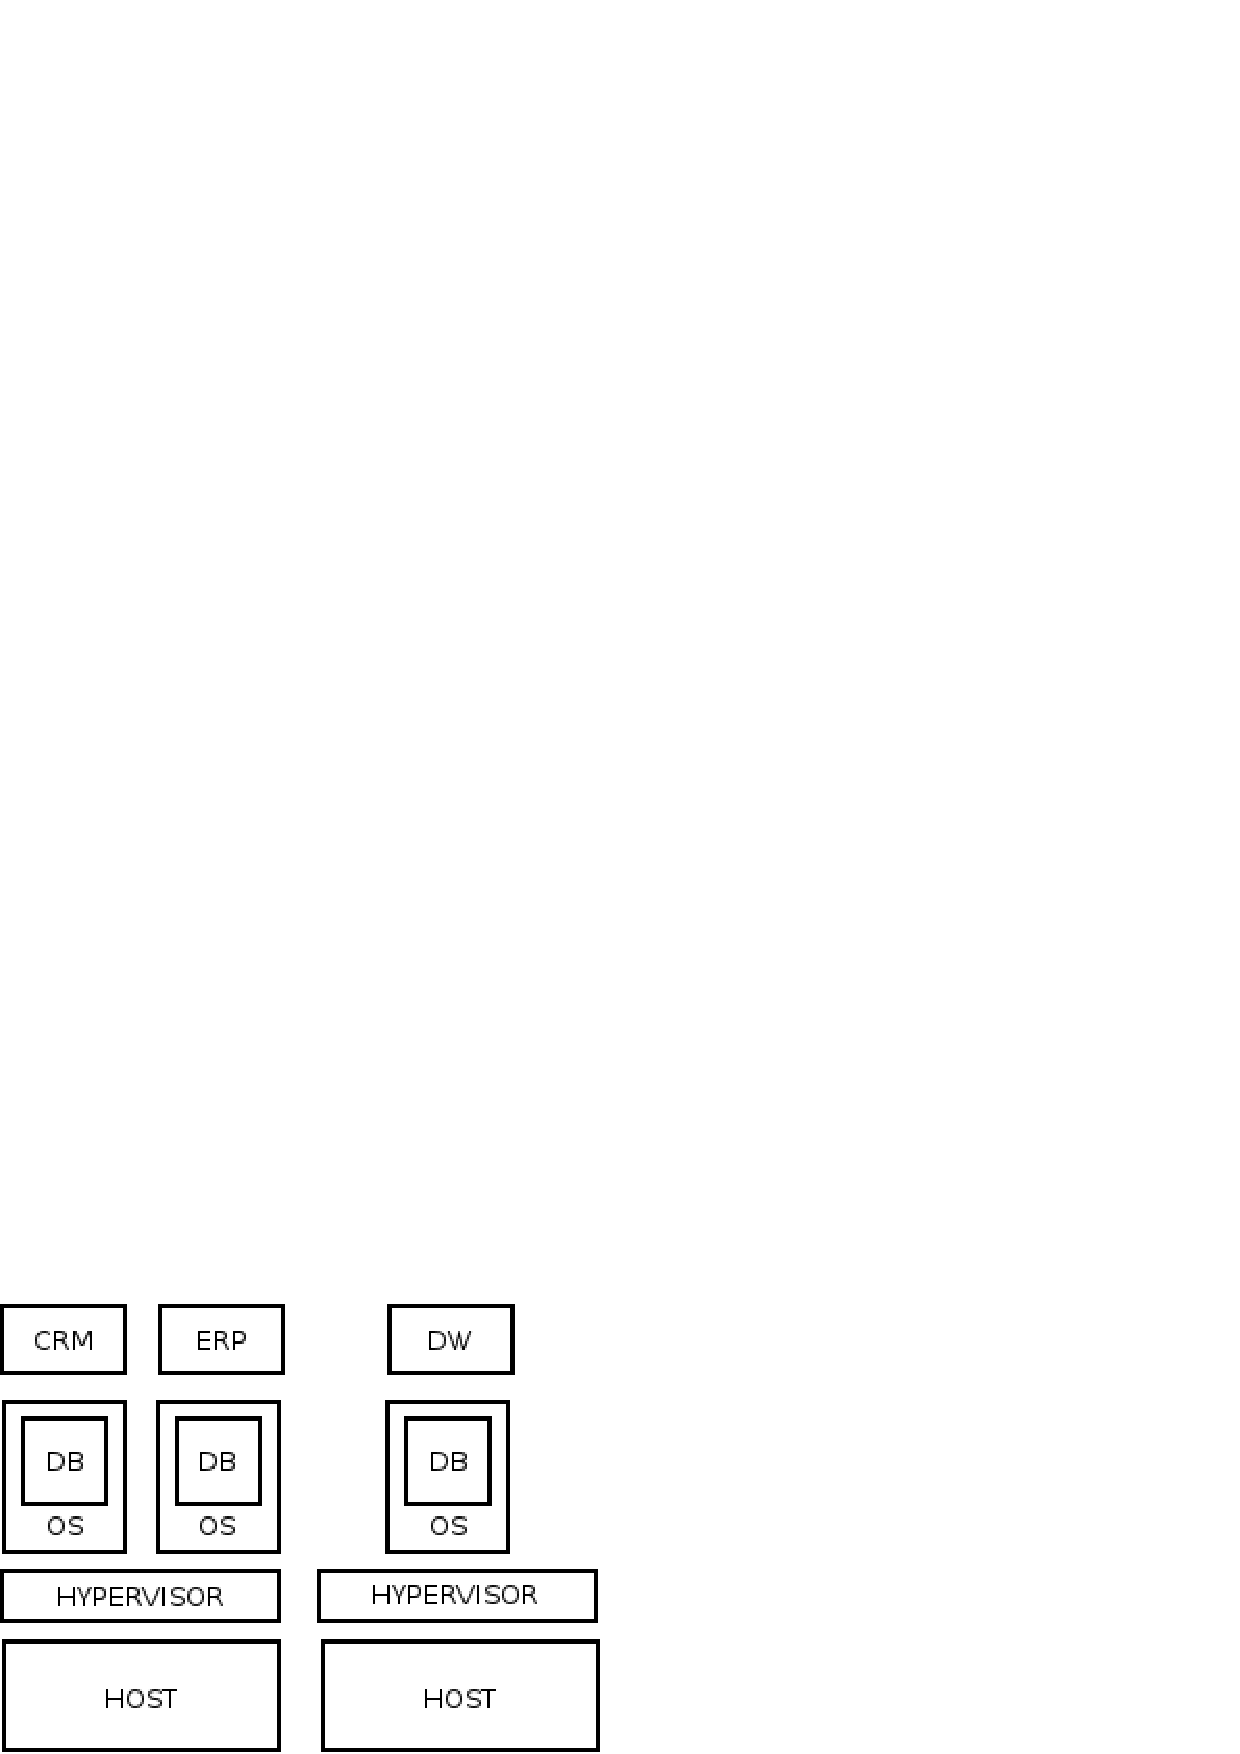
\includegraphics[width=0.5\textwidth]{infra-model.png}
	  \label{fig:infra-model}
	\end{figure} 

     
    \end{itemize}


  \end{frame}
   

\section{Objective}

\begin{frame}
 \frametitle{Objective}
 
 \begin{block}{Problem definition}%\cite{4401021}}
    \textit{"Given N database workloads that will run on N database systems inside N virtual 
machines, how should we allocate the available resources to these virtual machines to get the best overall performance?"}\cite{4401021}
 \end{block}
 \begin{figure}[ht]
      \centering
    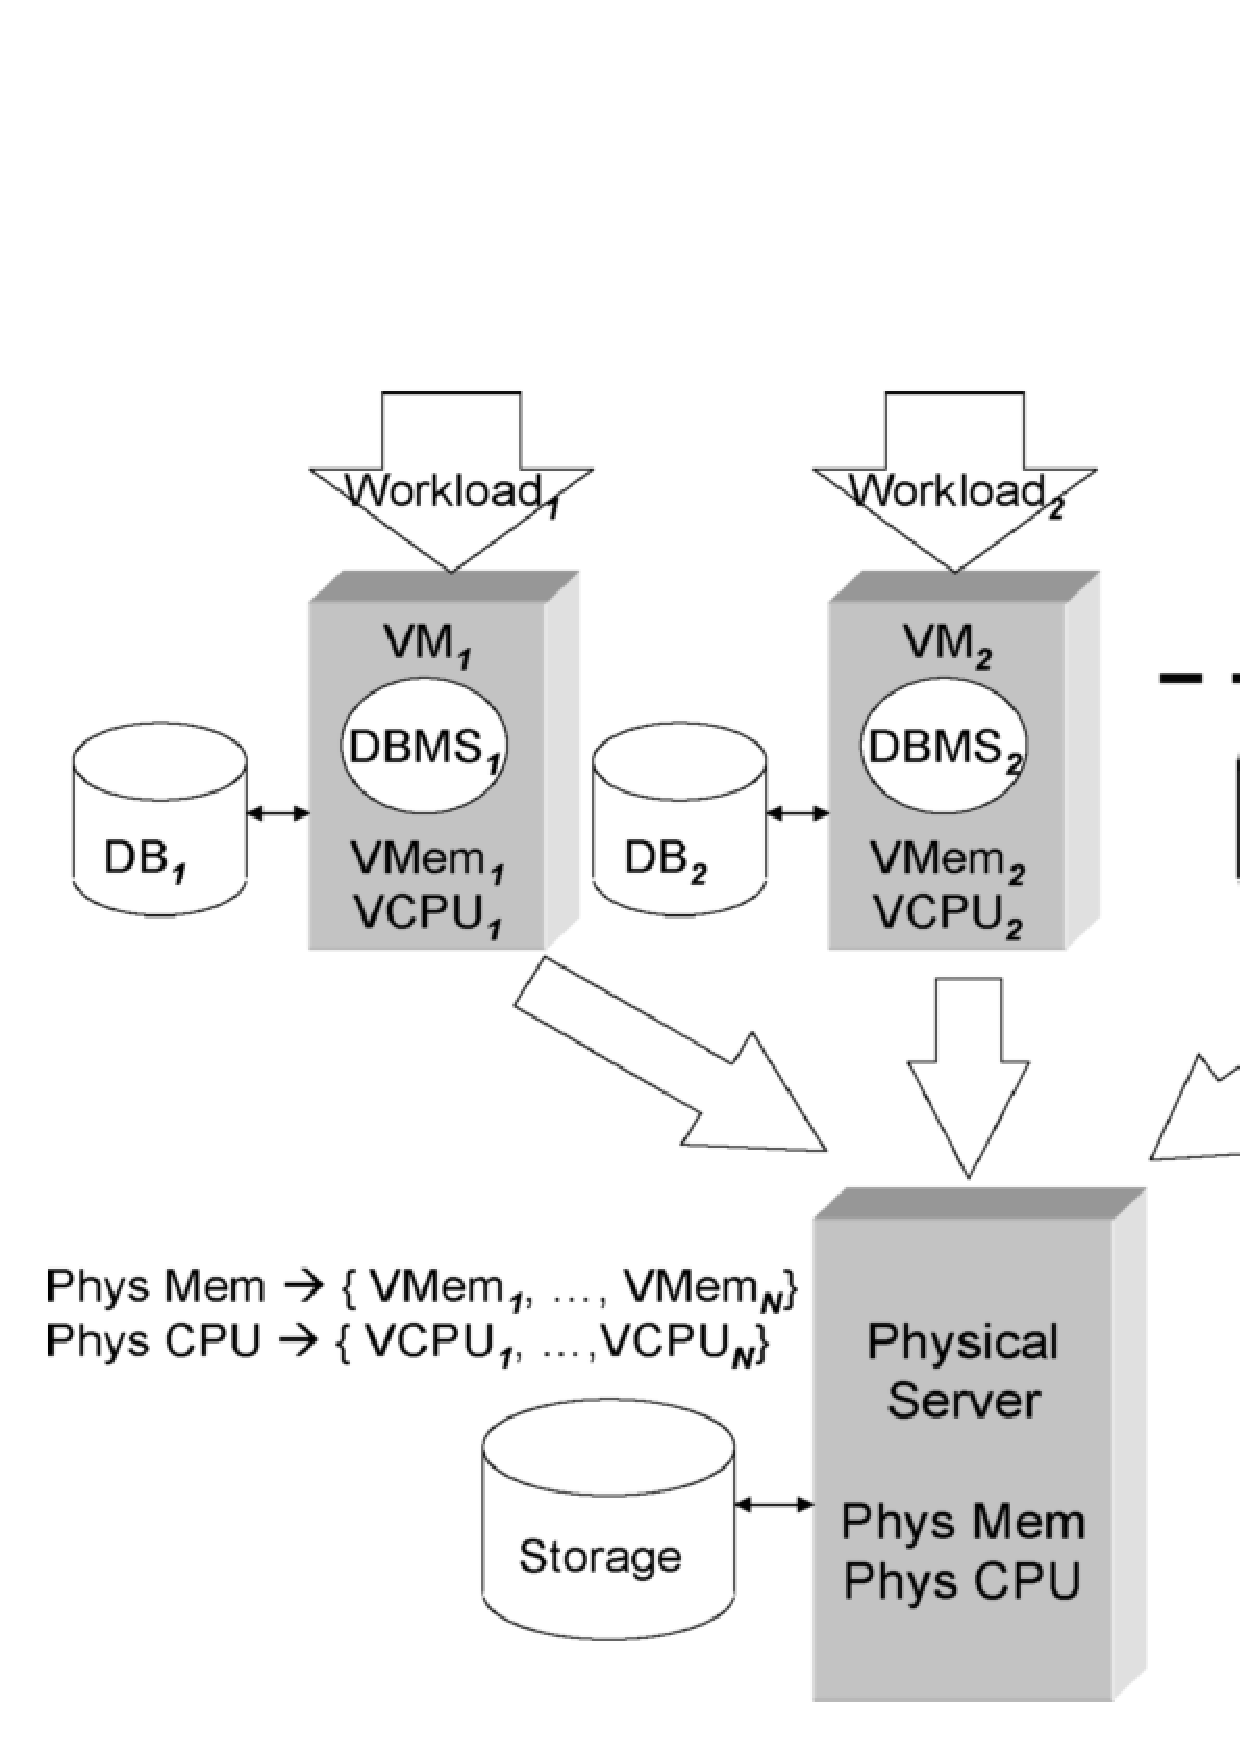
\includegraphics[width=0.4\textwidth]{dbms_consolidation.png}
    \caption{Resource Consolidation scenario}
    \label{fig:scenario}
\end{figure} 

  

\end{frame}

\section{Related Work}
\subsection{Overview}
  \begin{frame}
     
    \frametitle{Related Work}
    \begin{itemize}
     \item \cite{dias:automatic}
      \begin{itemize}
	\item CPU among distributes systems;
     \end{itemize}
     \item \cite{6127969}
      \begin{itemize}
	\item CPU virtualization overhead;
      \end{itemize}


     \item \cite{Soror:2008:AVM:1376616.1376711-OLD} and \cite{Soror:2008:AVM:1376616.1376711}
     \begin{itemize}
      \item CPU cost models;
      \item Virtualization design advisor;

     \end{itemize}

    \end{itemize}


  \end{frame}
  
 


\subsection{Virtualization Design Advisor}
  \begin{frame}
    \begin{itemize}
     \item Objective:
     \begin{itemize}
      \item Minimize $\sum_{i=1}^{N} Cost(W_{i},R_{i})$.
     \end{itemize}
     \begin{block}{Problem}
	$Cost_{DB}(Q,P_{i},D) \longrightarrow Cost(W_{i},R_{i})$
     \end{block}

    \end{itemize}
   
  \end{frame}
  
  \begin{frame}
  \frametitle{Cost estimator overview}
   \begin{figure}[ht]
      \centering
      \includegraphics[width=0.5\textwidth]{cost-estimator.png}
      \caption{Cost estimator overview}
      \label{fig:architecture}
    \end{figure} 
  \end{frame}


  \begin{frame}
    \frametitle{Advisor overview}
    \begin{figure}[ht]
      \centering
      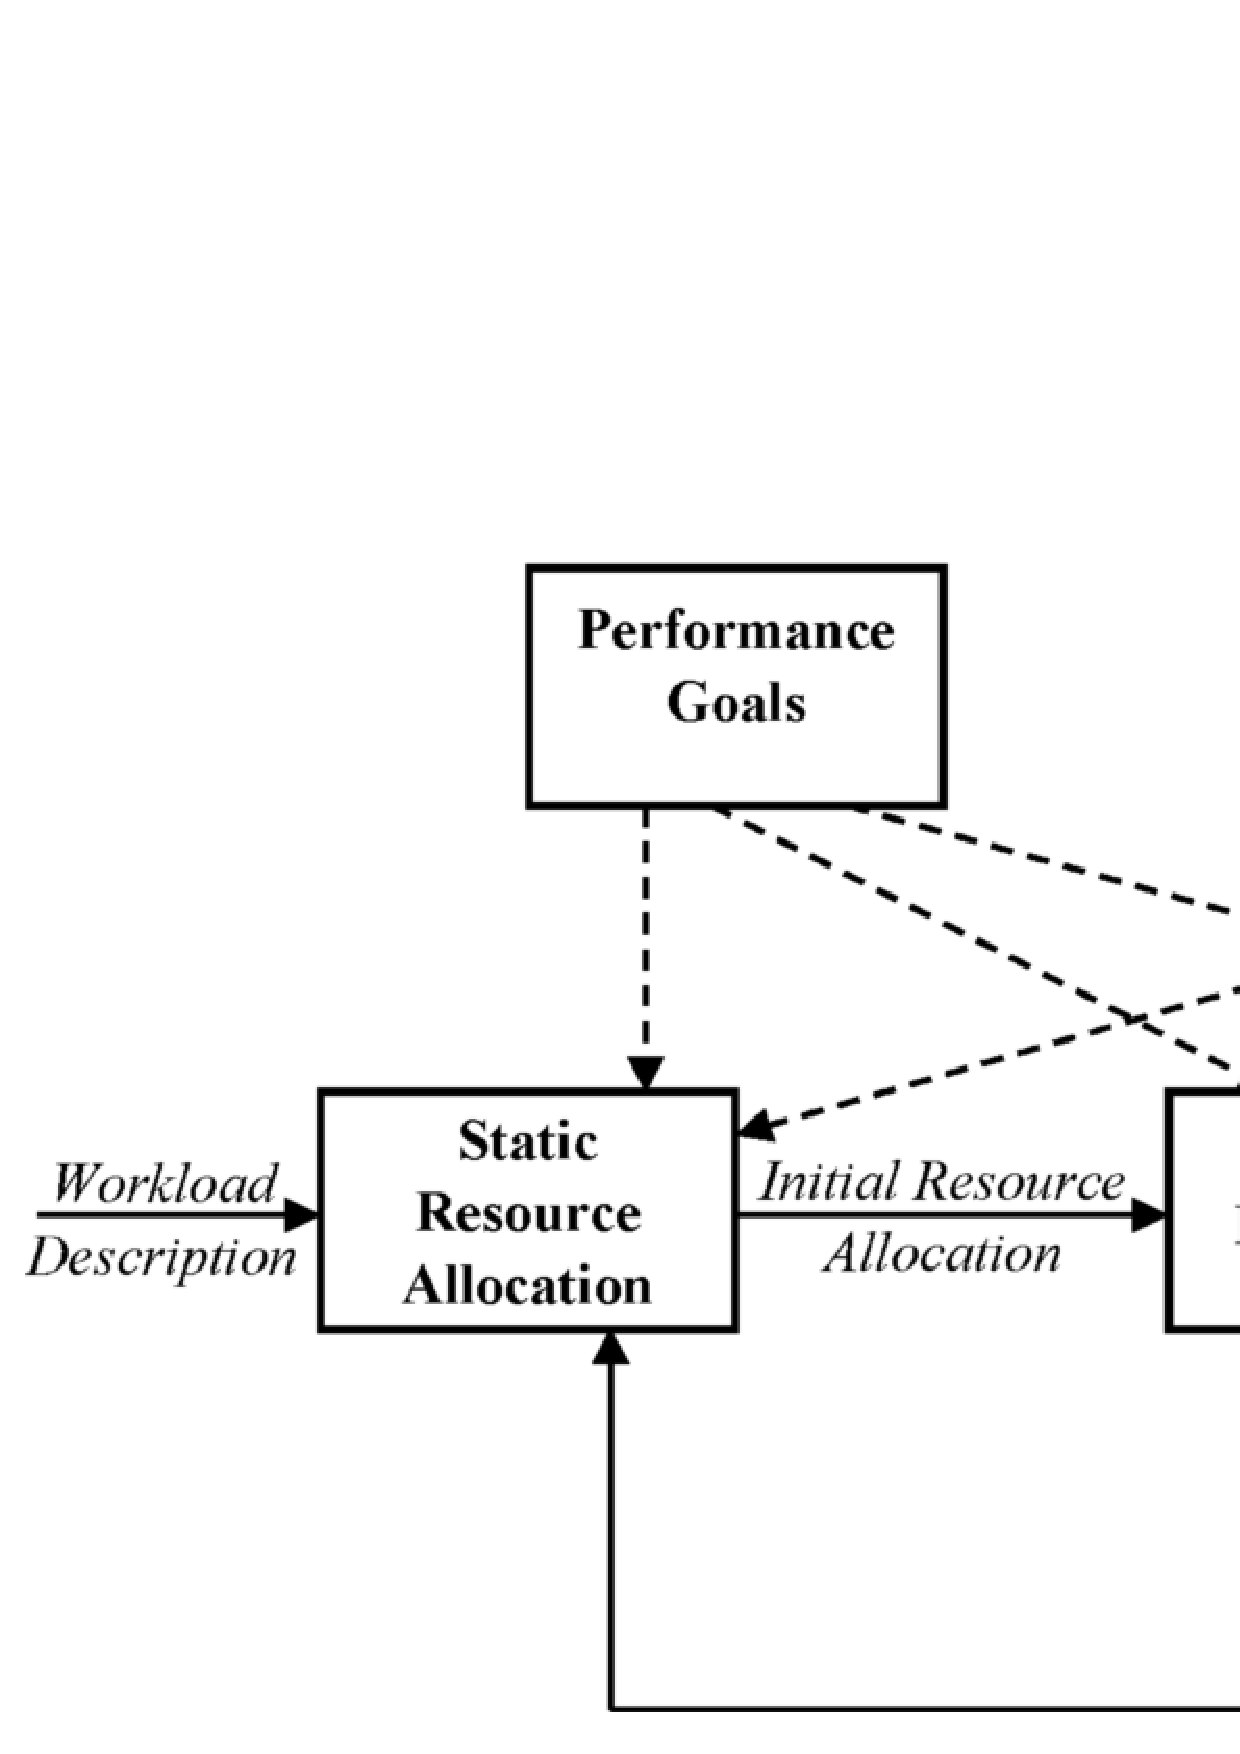
\includegraphics[width=0.8\textwidth]{architecture.png}
      \caption{Advisor overview}
      \label{fig:architecture}
    \end{figure} 

  \end{frame}
  
\section{Solution}

\subsection{OpenNebula}
  \begin{frame}[plain]
    \frametitle{OpenNebula}
    \begin{itemize}
     \item Homogeneous view of resources;
     \item Manages VM full life cycle;
     \item Configurable resource allocation policies;
    \end{itemize}
    
    \begin{figure}[ht]
      \centering
      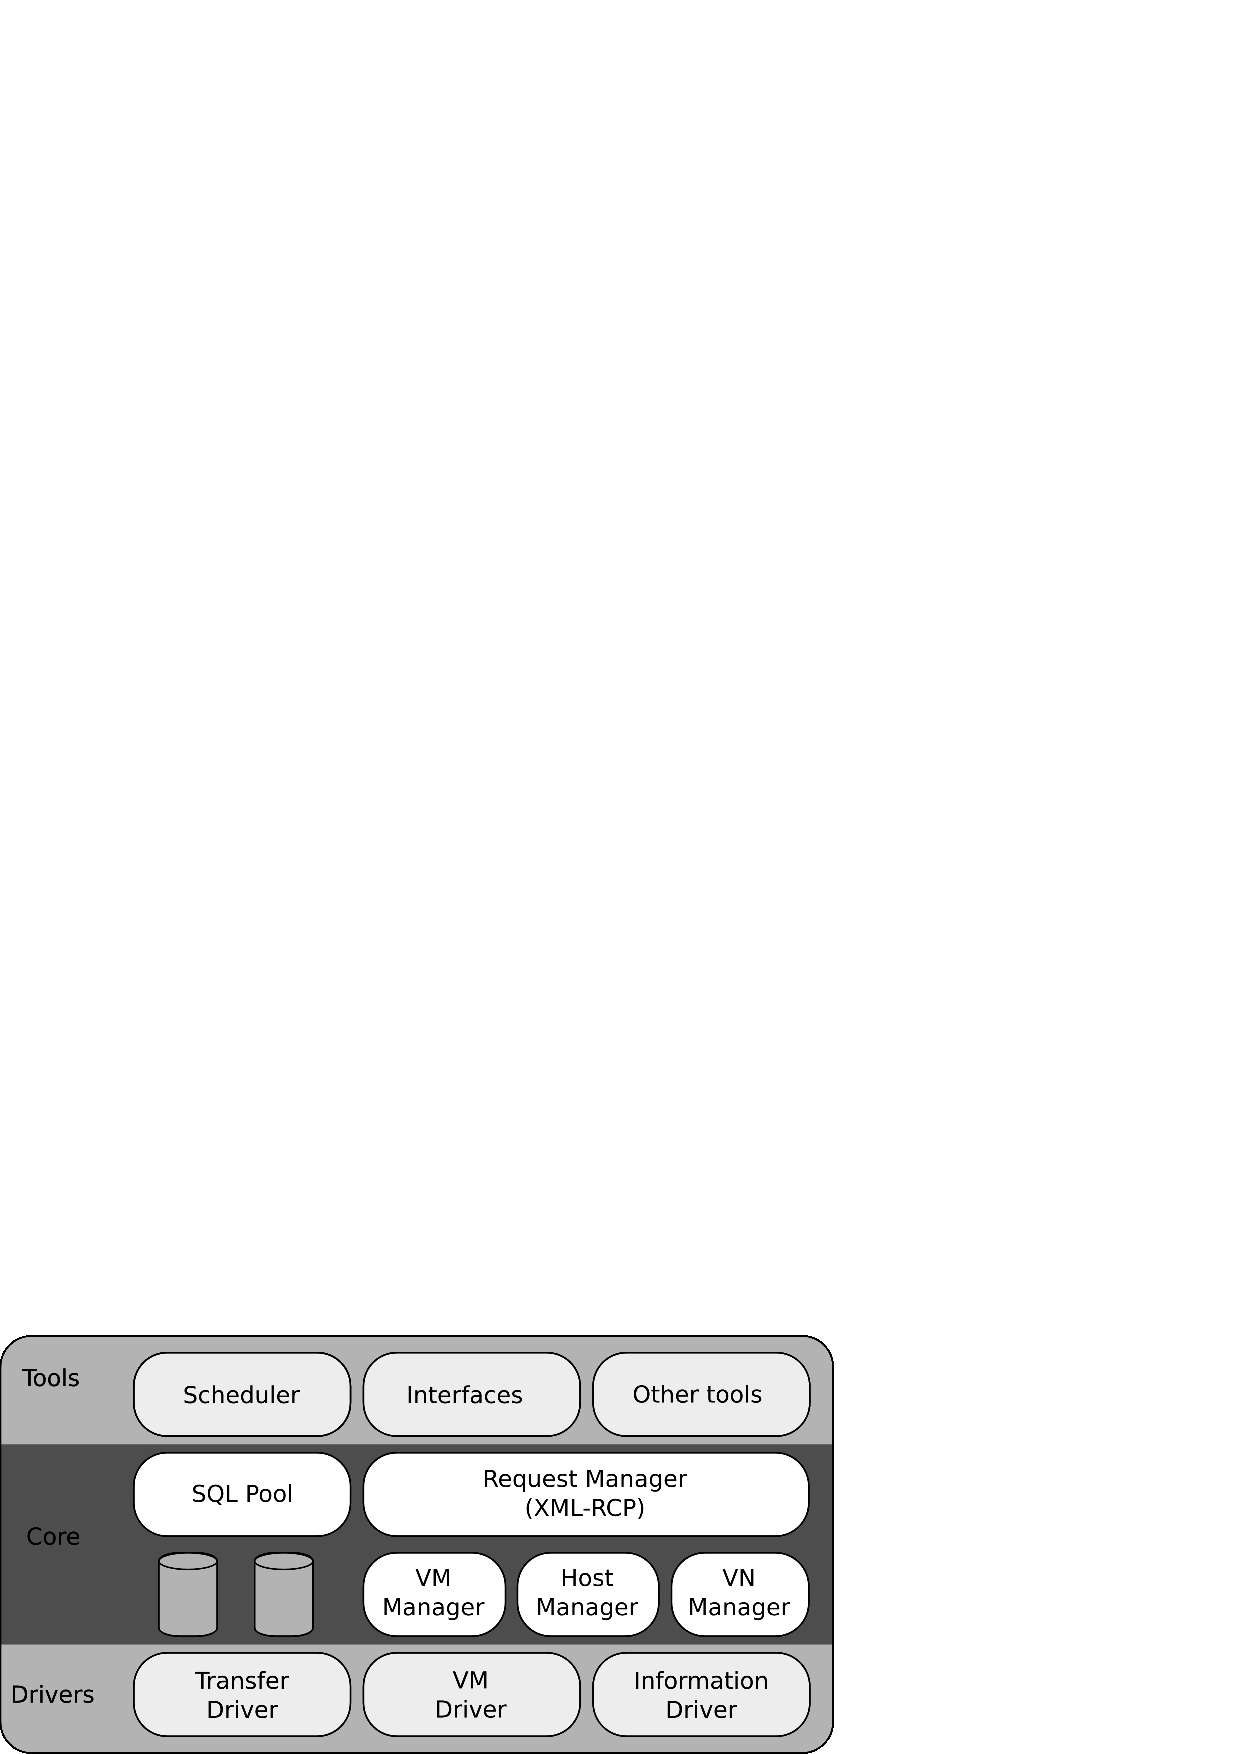
\includegraphics[scale=0.5]{one-architecture_2.png}
      \caption{OpenNebula architecture}
      \label{fig:open_arch}
    \end{figure}


  \end{frame}
  

  
  \subsection{OpenRC}
  \begin{frame}
    \frametitle{OpenRC}
     \begin{itemize}
      \item Advisor implementation for a private cloud;
      \item Supporting features.
      \begin{itemize}
       \item Resource reallocation;
       \item Communication with the DBMS:
       \begin{figure}[ht]
	  \centering
	  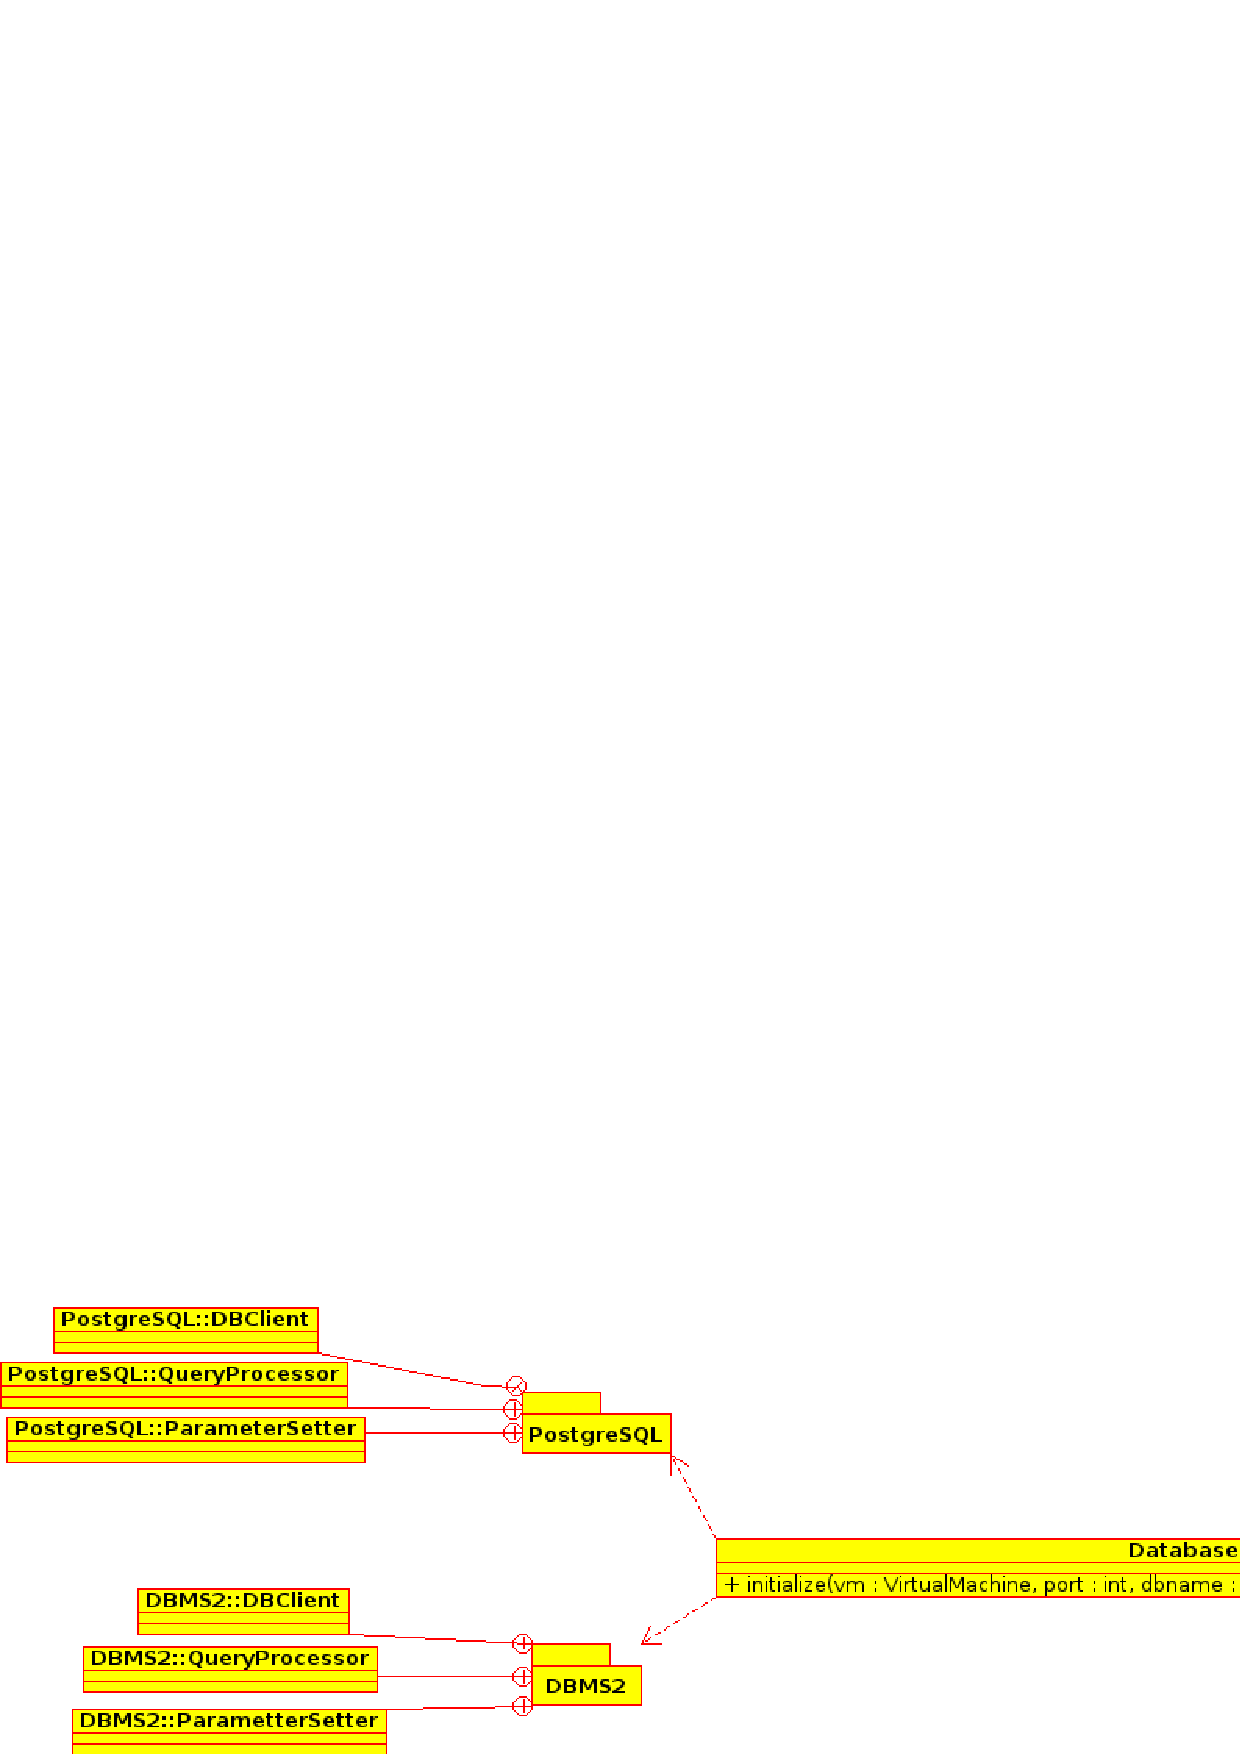
\includegraphics[scale=0.3]{database_helper_facade.png}
	  \label{fig:facade}
	\end{figure}
      \end{itemize}

     \end{itemize}
  \end{frame}
  
  \begin{frame}
   \frametitle{Calibration and renormalization}
 
   Parameters that describe CPU:

      \begin{table}[ht]
	\centering
	\scalebox{0.5}{
	  \begin{tabular}{ | l | p{5cm} |}
	    \hline
	    Parameter & Description  \\ \hline
	    \textbf{cpu\_operator\_cost} & Cost of processing each operator or function call \\ \hline
	    \textbf{cpu\_tuple\_cost} & Cost of processing one tuple (row) \\ \hline
	    \textbf{cpu\_index\_tuple\_cost} & Cost of processing each index entry during an index scan  \\
	    \hline
	  \end{tabular}
	}	
	%\caption{Parameters that describe CPU}
	\label{table:descriptive}
      \end{table}
      Normalization in PostgreSQL:
	\begin{itemize}
	\item \textbf{seq\_page\_cost}: Cost of fetching a sequential page from disk.
      \end{itemize}

      Relation between costs:
      \[
	  param_{estimated} = \frac{param_{actual}}{seq\_page\_cost_{actual}}
      \]
  \end{frame}
  
  \begin{frame}
   \frametitle{Implementation Overview}
   \begin{figure}[ht]
      \centering
      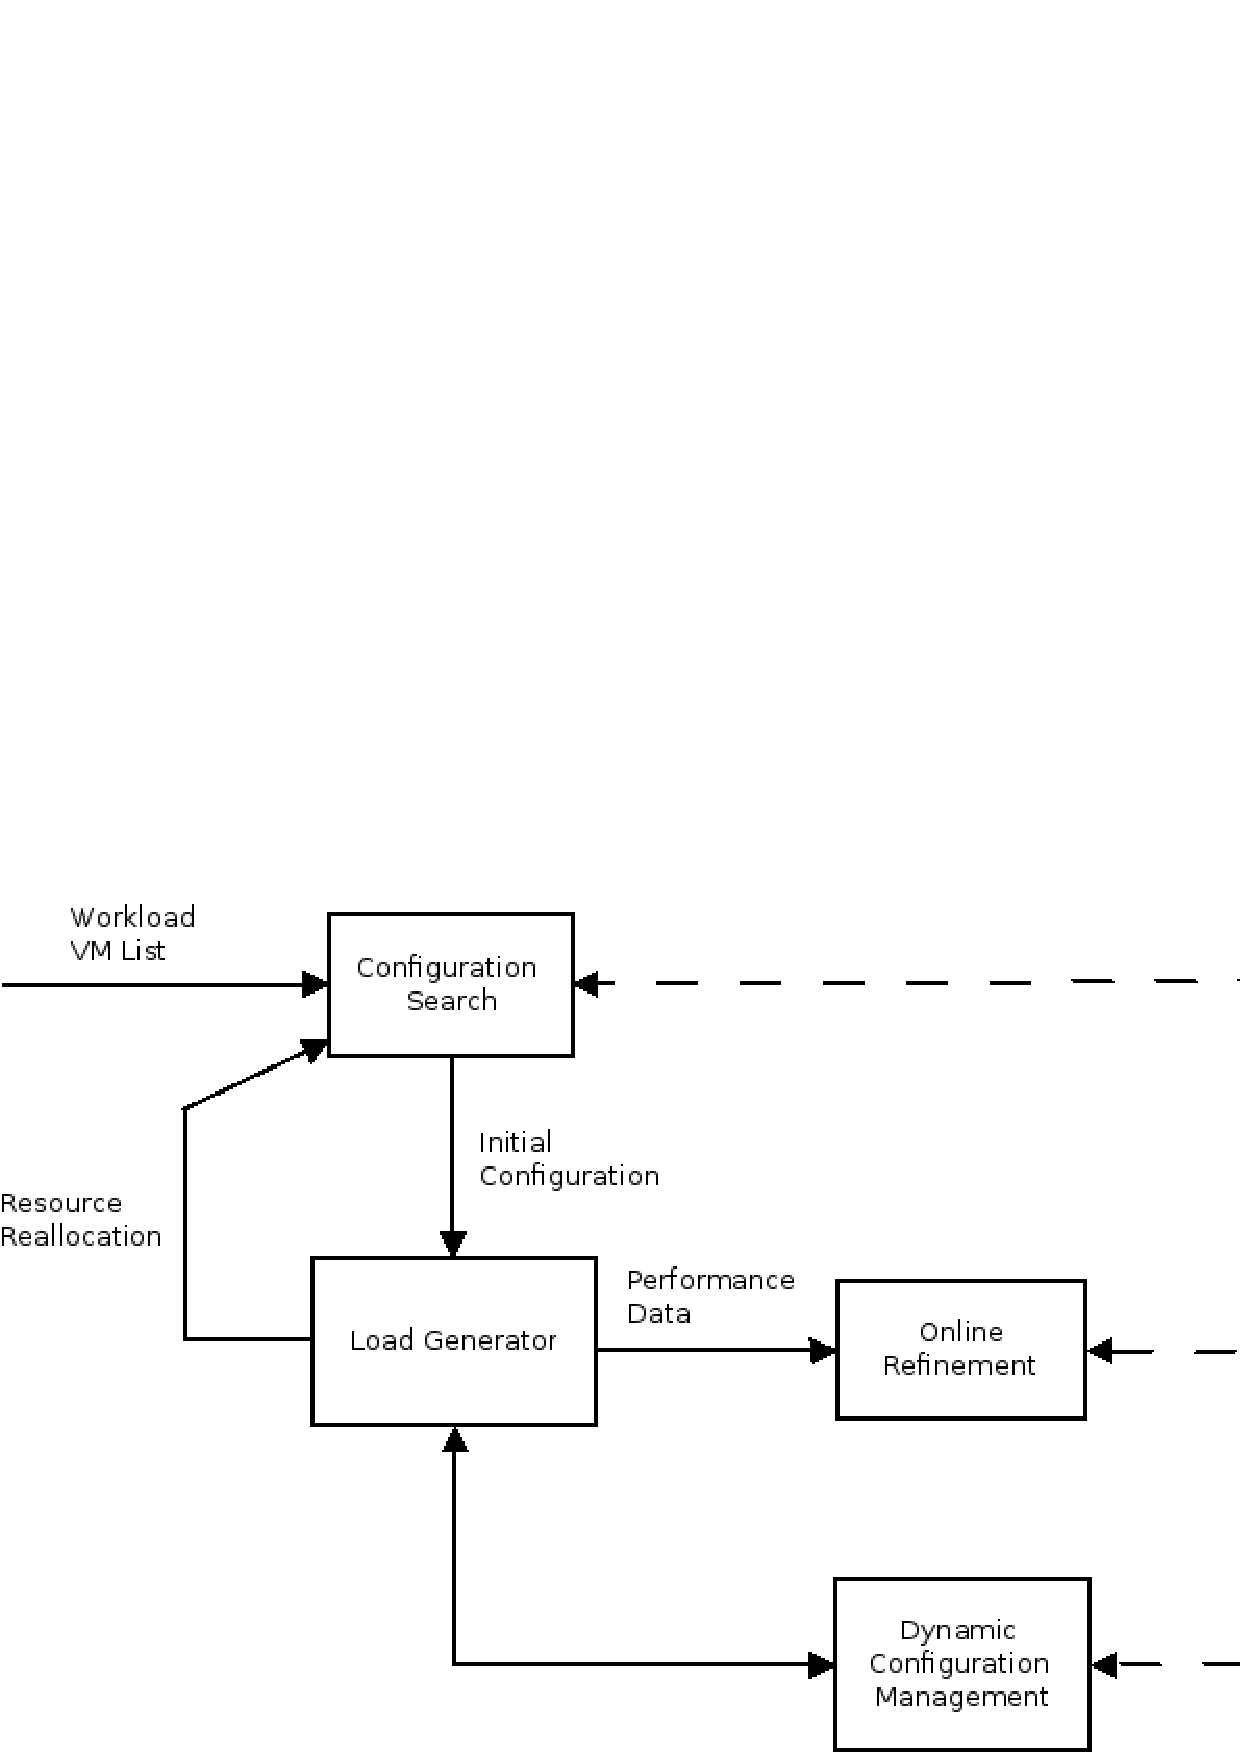
\includegraphics[width=0.8\textwidth]{advisor-arch.png}
      \caption{Implementation overview}
    \end{figure} 
  \end{frame}


  
      
\section{Results}
  \begin{frame}
    \frametitle{Calibration}
    \begin{columns}
    \begin{column}{0.3\textwidth}
      \centering
      \includegraphics[width = 4 cm]{cpu-operator-cost.png}
    \end{column}
    \begin{column}{0.3\textwidth}
      \centering
      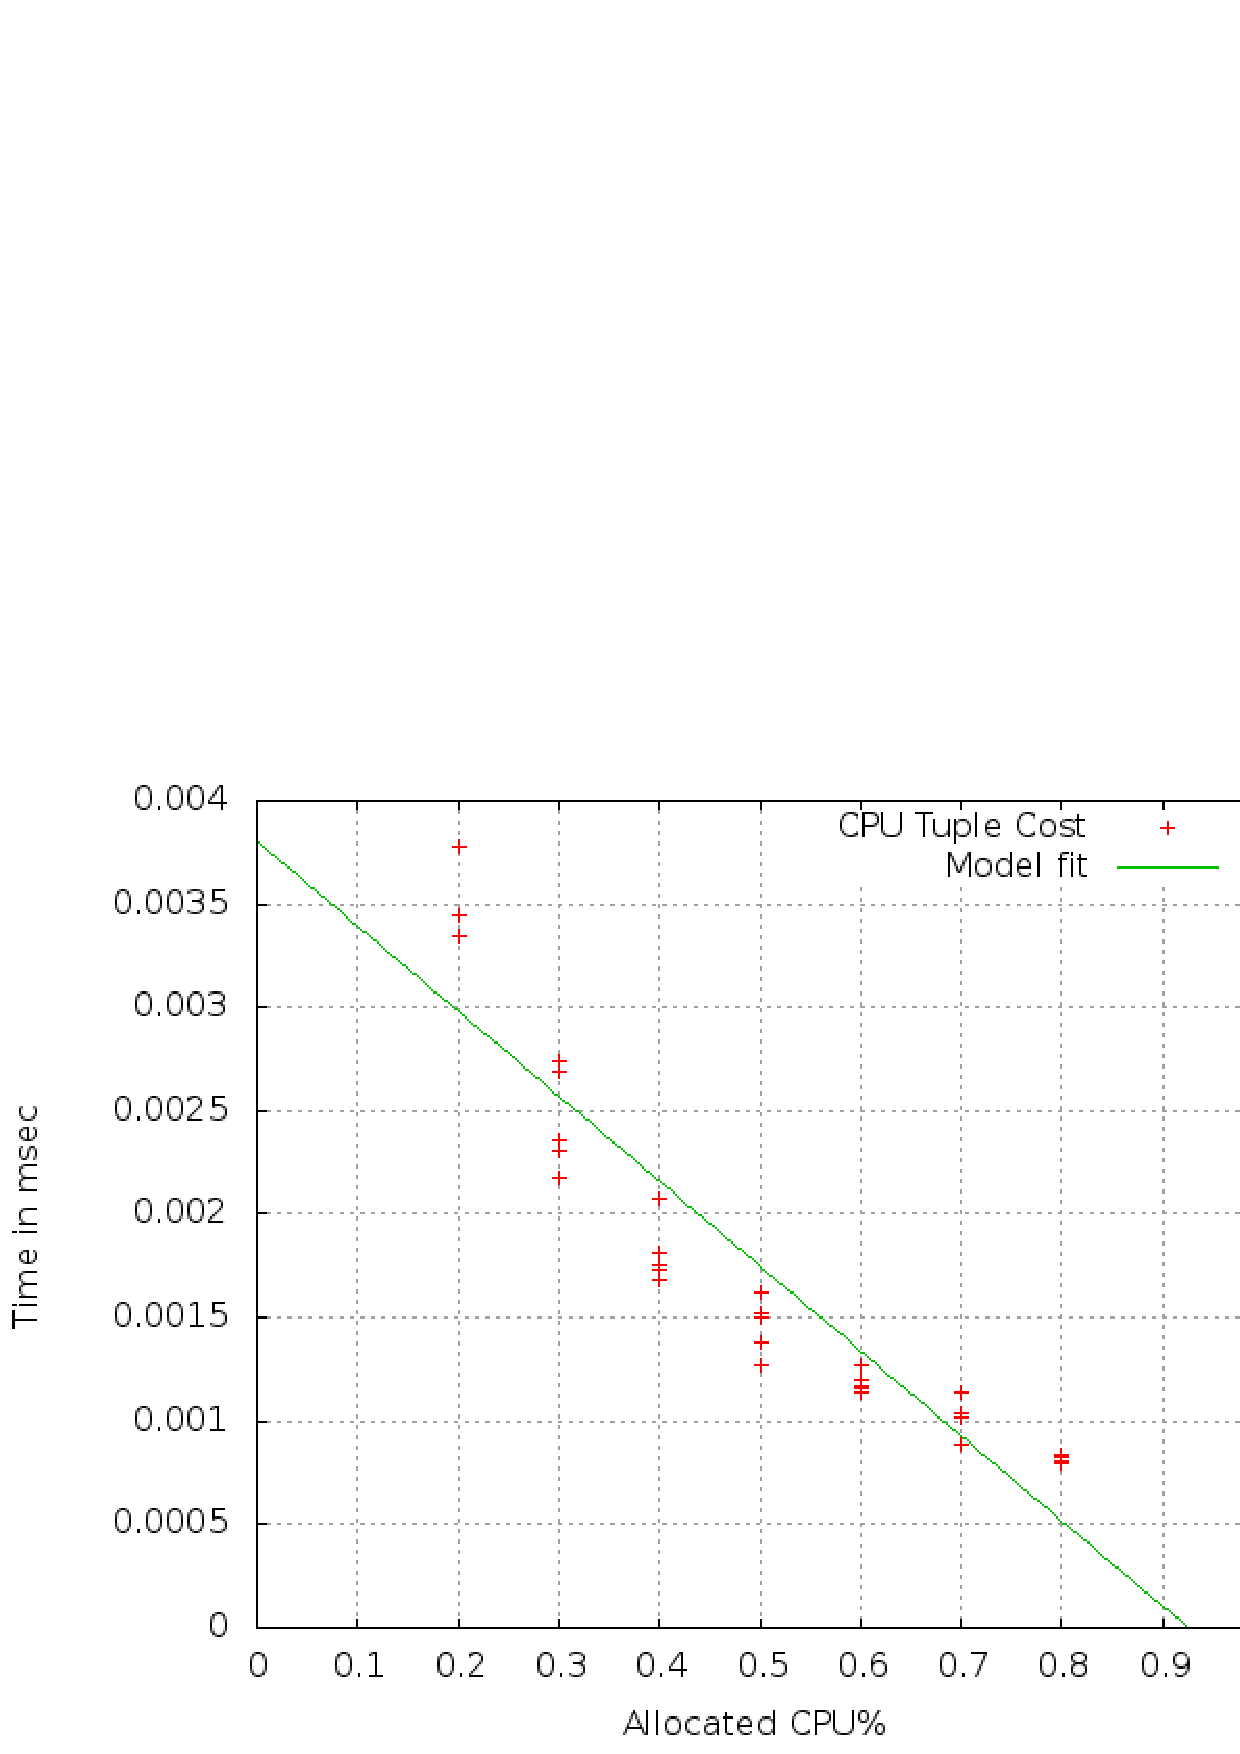
\includegraphics[width = 4 cm]{cpu-tuple-cost.png}
    \end{column}
    \begin{column}{0.3\textwidth}
      \centering
      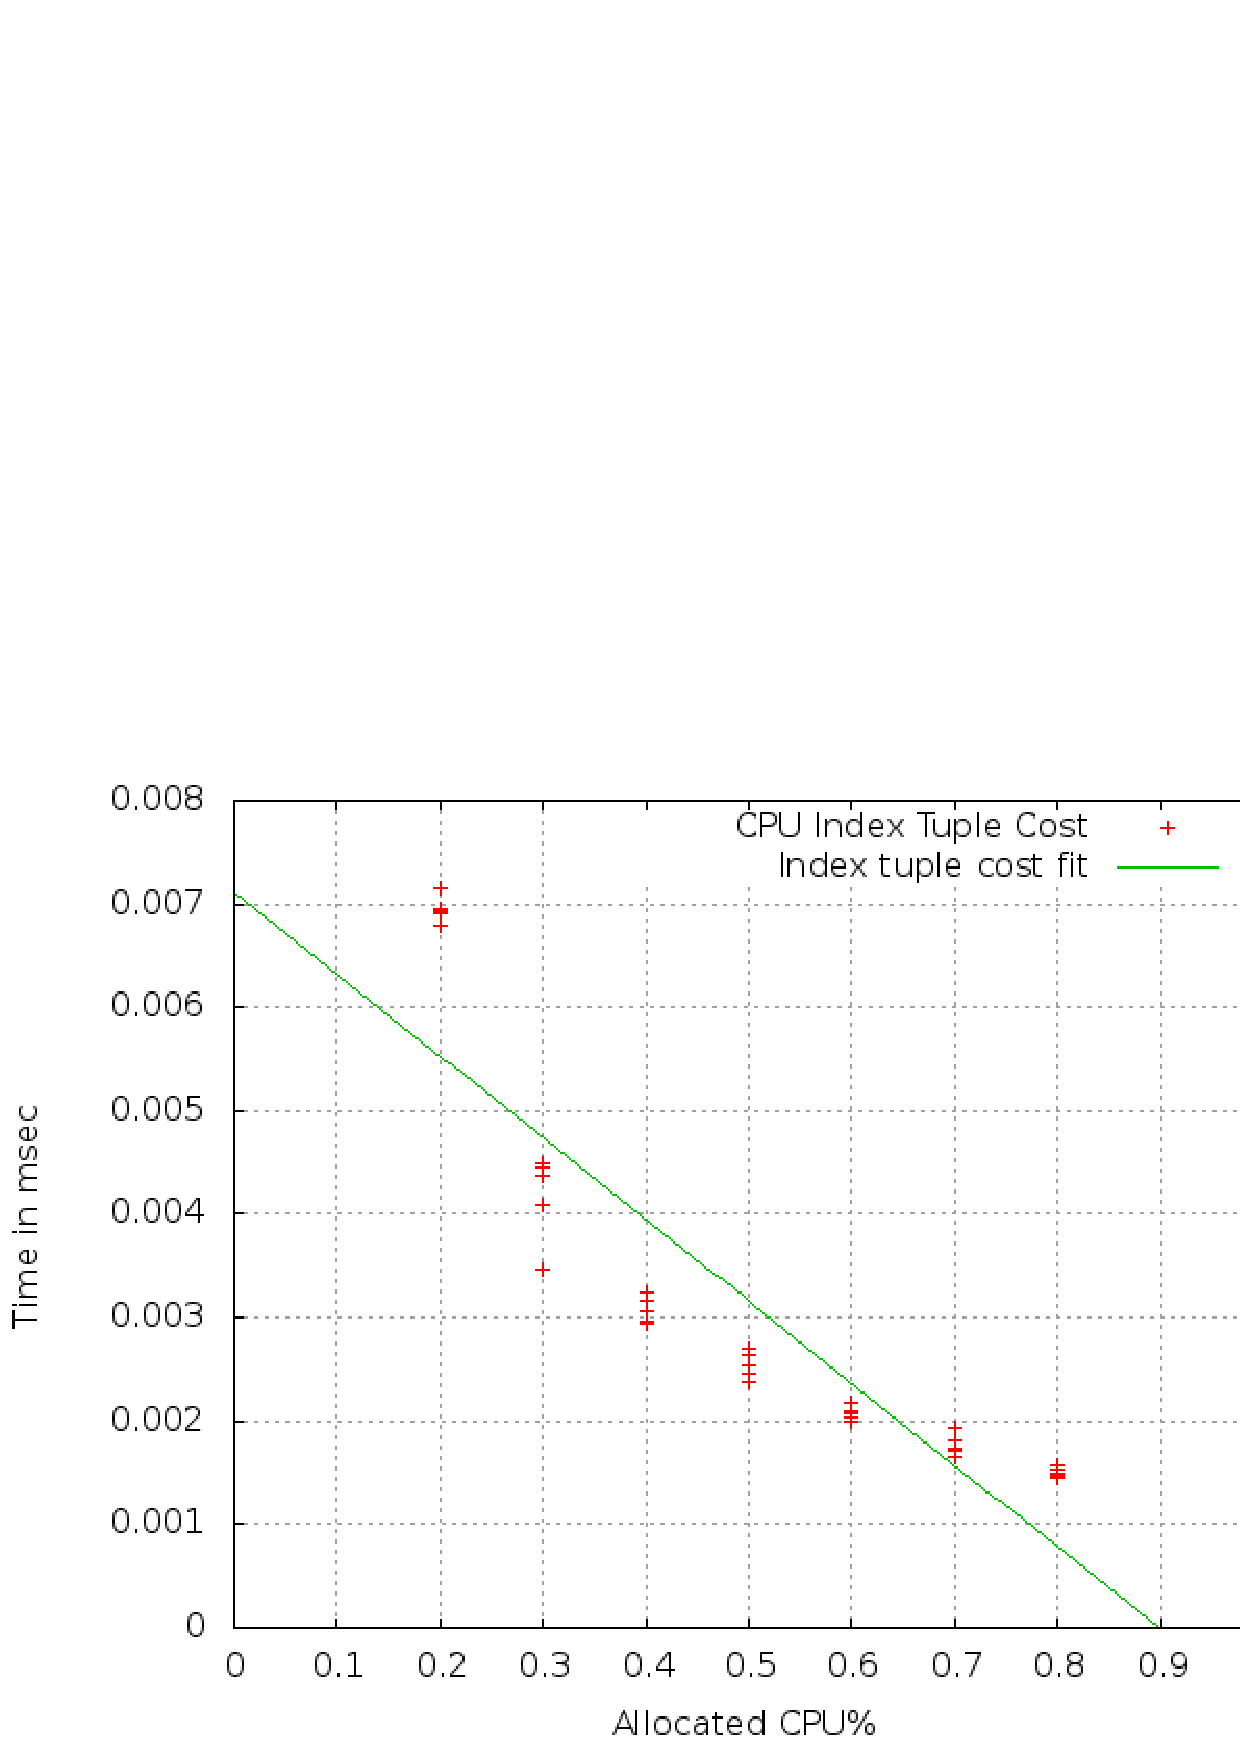
\includegraphics[width = 4 cm]{cpu-index-tuple-cost.png}
    \end{column}
  \end{columns}

  \end{frame}

\subsection{Advisor}

  \begin{frame}
    \frametitle{Configuration Search}
    \begin{columns}
    \begin{column}{0.6\textwidth}
      \centering
          \[
      \frac{T_{default}-T_{advisor}}{T_{default}}
      \]
      \begin{eqnarray*}
	W_{1} &=& 5*C + 5*I \\
	W_{2} &=& k*C + (10-k)*I, \\
	  &&0 \leq k \leq 10 \\
      \end{eqnarray*}
    \end{column}
    \begin{column}{0.6\textwidth}
      \centering
      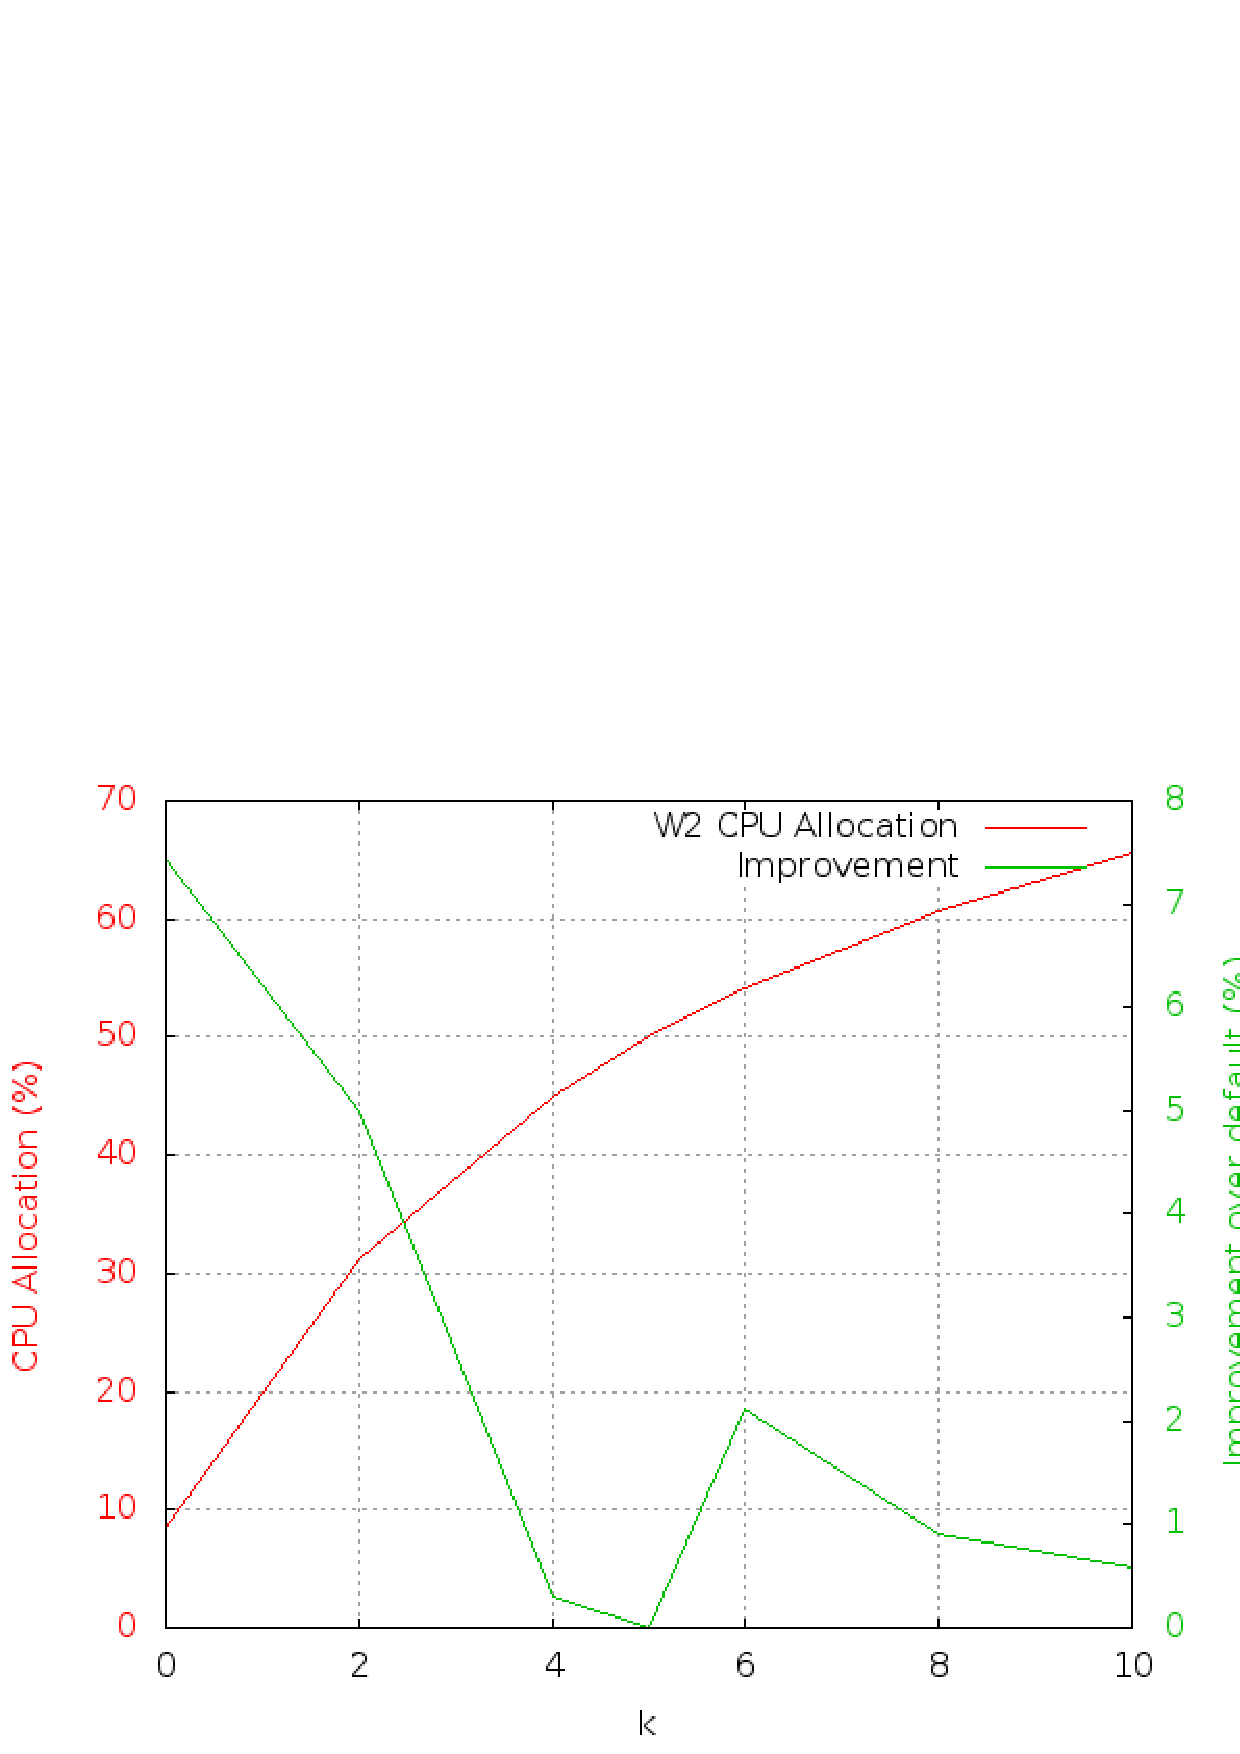
\includegraphics[width=0.8\textwidth]{improvement.png}
    \end{column}
      \end{columns}

  \end{frame}

\begin{frame}
    \frametitle{Online Refinement and Dynamic Configuration Search}
    \begin{columns}
    \begin{column}{0.6\textwidth}
      \centering
	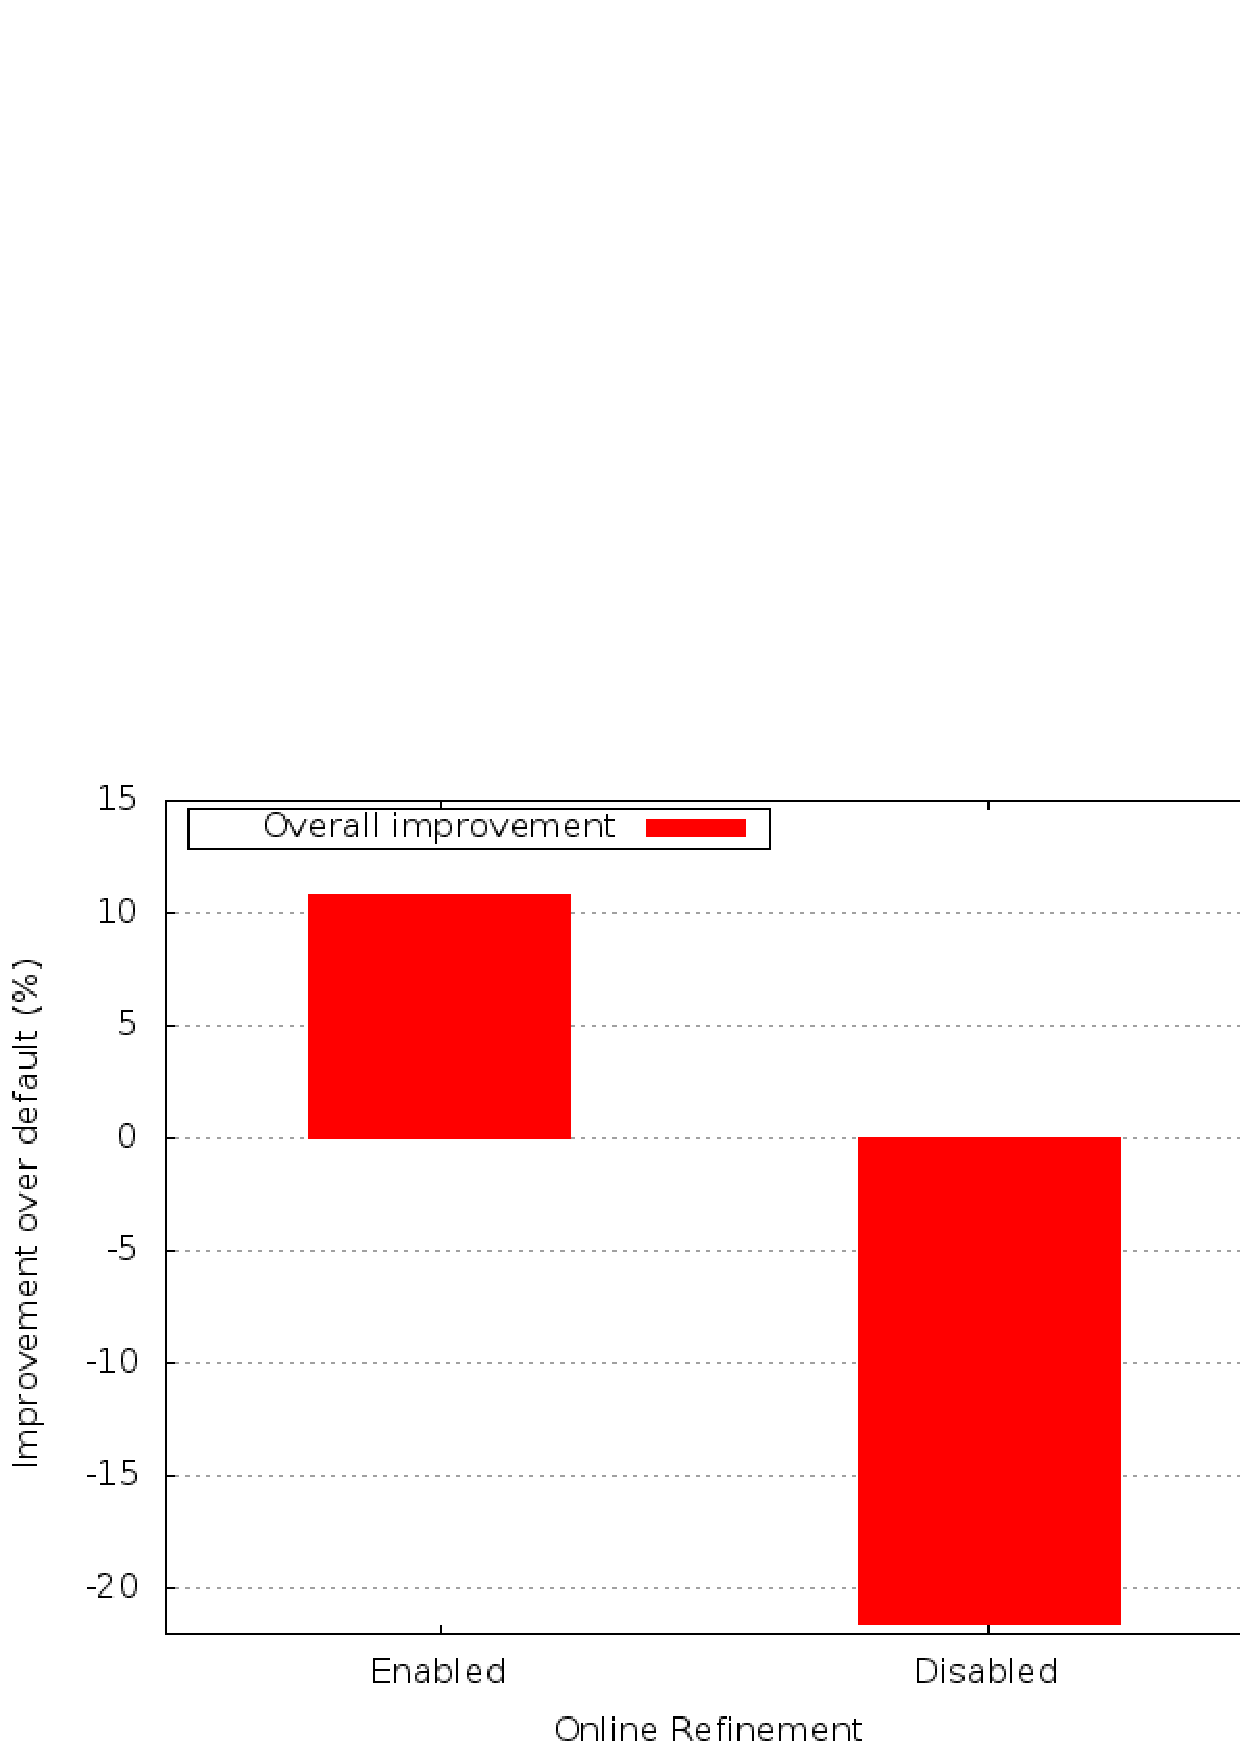
\includegraphics[width=0.8\textwidth]{online-ref.png}
    \end{column}
    \begin{column}{0.6\textwidth}
      \centering
  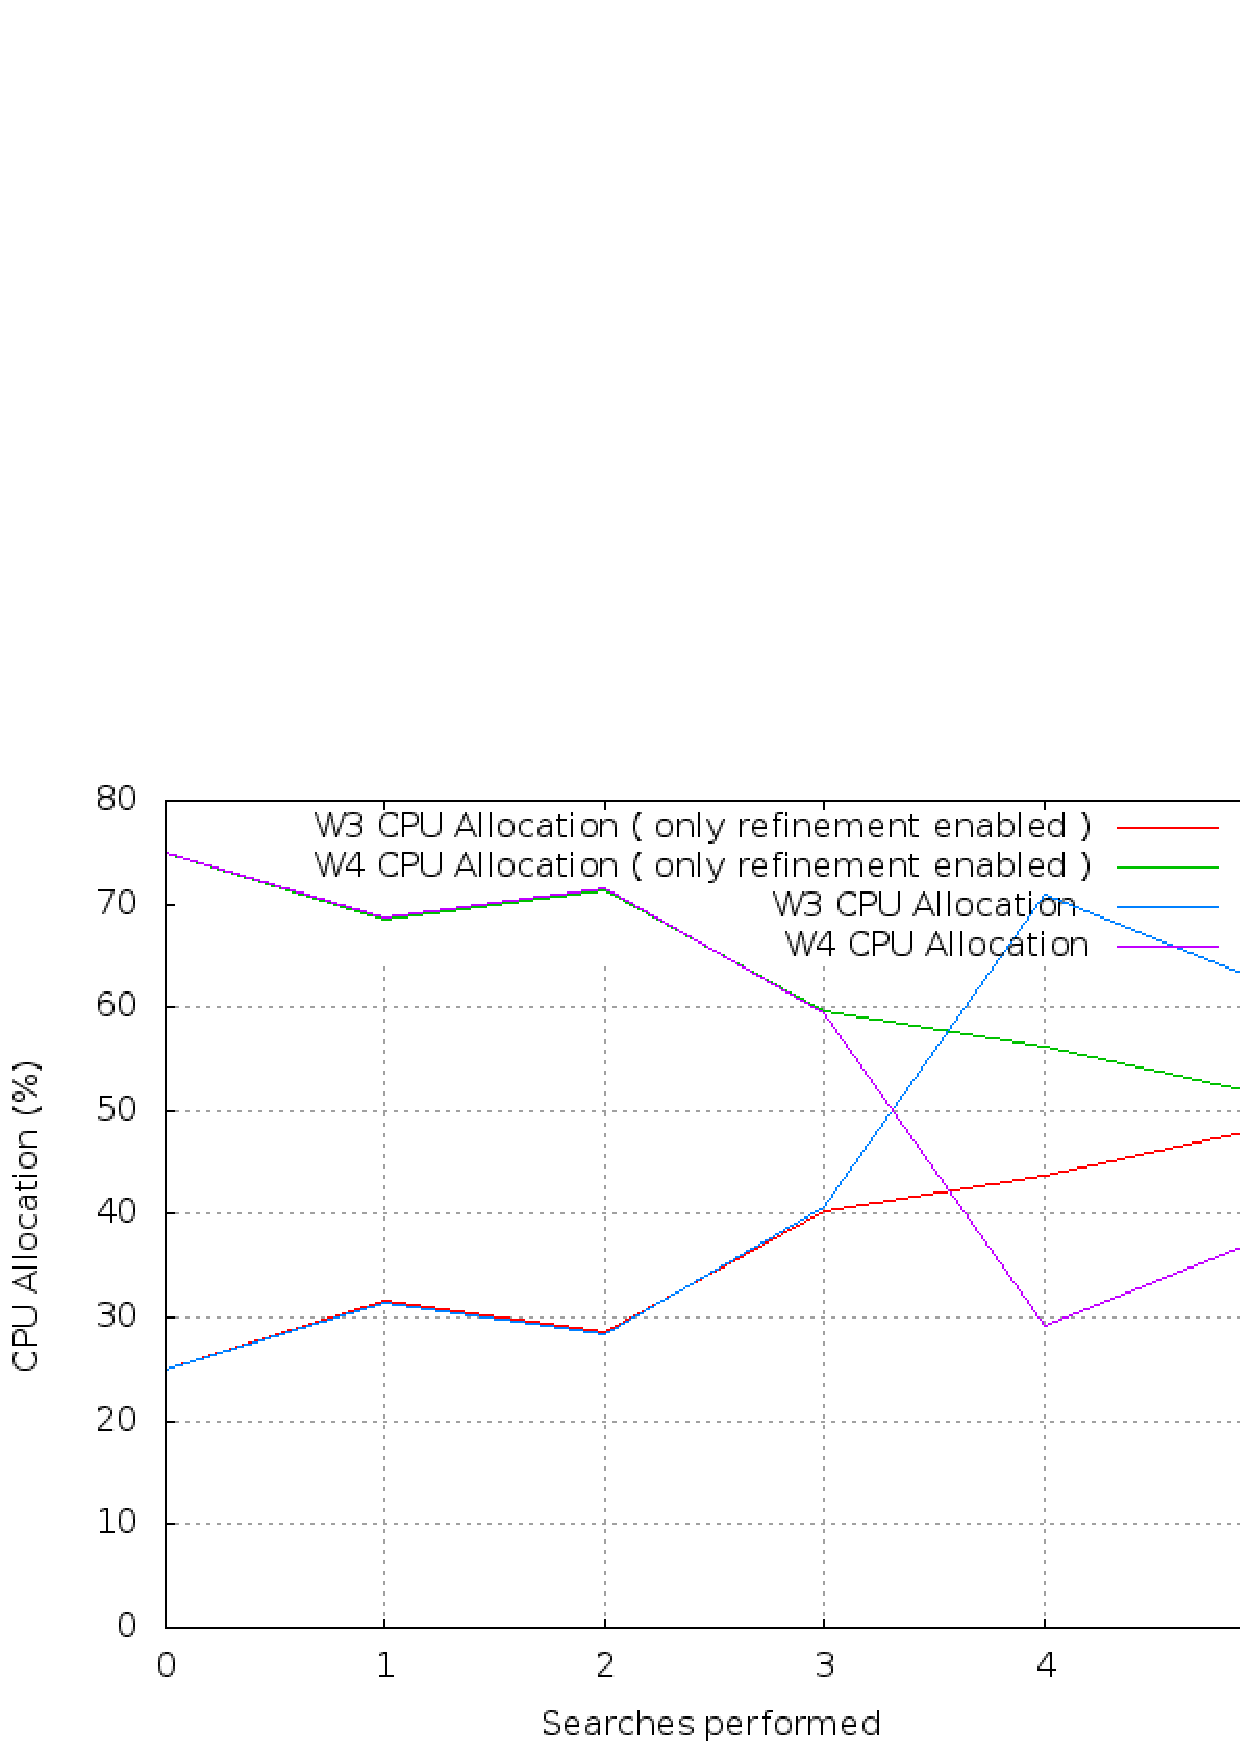
\includegraphics[width=0.8\textwidth]{dyn-change.png}
    \end{column}
      \end{columns}

  \end{frame}

\section{Final Considerations}
  \begin{frame}
      \frametitle{Final Considerations}
      \begin{itemize}
       \item Resource consolidation in the cloud;
       \item Improvement over default allocation;
       \item Future work
       \begin{itemize}
	  \item Different DBMS types;
	  \item New resources;
	  \item Explore the infrastructure;
	  \item Overhead;
       \end{itemize}

      \end{itemize}


  \end{frame}
 
 \section{References}


\nocite{*}
\bibliographystyle{apalike}
\bibliography{tg}




\end{document}
